\section{\ExT: A DSL for Document Authoring} \label{sec:dsl}

We have presented the advantages of compositional embeddings using a relatively
small DSL. One may wonder if our approach scales to larger DSLs. As our answer
to this question, we developed a larger DSL for document authoring called \ExT
(\emph{EXtensible Typesetting}).

\ExT applies compositional embeddings to a document DSL, inspired by \LaTeX{}
and Scribble~\citep{flatt2009scribble}. We have also done minor syntactic
extensions to the CP language to support writing documents more naturally. Since
documents usually involve large portions of text, it would be awkward to write
such portions of text using string literals adopted by most programming
languages. CP does not yet have facilities for syntactic extension that other
languages (e.g. Racket, Haskell, or Coq) offer, so we have extended the parser
directly. Thus, CP parses some document-specific syntax and desugars it to
compositionally embedded fragments during parsing. Such a generative approach is
similar to Racket macros~\citep{ballantyne2020macros} and Template
Haskell~\citep{sheard2002template}, which provide more flexible facilities for
performing such desugaring. Nevertheless, the surface syntax of \ExT is
essentially a set of lightweight syntactic sugar for its underlying
compositional embeddings (similar, for instance, to Scribble in Racket).

\subsection{Design Goals and Non-Goals} \label{sec:goals}

There are already a large number of document DSLs, so why shall we create yet
another one? We explain why by identifying important design goals and non-goals
of \ExT.

\paragraph{A document language for the web.}
A first goal is to have a lightweight but powerful document language tailored
mostly for the web. We view \ExT as an alternative to Wikitext~\citep{wikitext},
the markup language used by Wikipedia, which shares similar goals. Similar to
Wikipedia pages, users can directly edit \ExT documents on a web page. But
different from Parsoid~\citep{parsoid}, the official Wikitext parser that runs
on the server side, our implementation can directly render documents on the
browser side.

\paragraph{General-purpose computation.}
The majority of existing document DSLs (e.g. CommonMark~\citep{mark},
Textile~\citep{textile}, and reStructuredText~\citep{rst}) have a fixed set of
language features and do not provide general-purpose computation. For instance,
we may want to compute a table from some data, like a table listing the largest
cities in descending order of population. For such kinds of tasks, it is useful
to have mechanisms for general-purpose computation that allow us to
\emph{compute} documents rather than manually write them.

Although some other document DSLs provide language constructs that enable some
computation, they still have significant limitations. For instance, Wikitext
provides templates, which play a role similar to functions in conventional
programming languages. However, templates cannot perform arbitrary computation
as CP does. The documentation says,\footnote{The sentence is extracted from
\url{https://en.wikipedia.org/wiki/Wikipedia:TEMPLATE_LOOP}.} ``A template can
call itself but will stop after one iteration to prevent an infinite loop.'' In
other words, templates by themselves are incapable of recursion or loops, but in
practice, loops are often needed in Wikipedia. For instance,
\lstinline|{{loop}}| has been used on approximately 99,000 pages.\footnote{The
number of transclusions (99,000 as of July 2022) is shown at
\url{https://en.wikipedia.org/wiki/Template:Loop}.} A Lua extension was
introduced to bypass such restrictions, and the widely-used template
\lstinline|{{loop}}| invokes \lstinline{string.rep} in Lua. Instead of handing
it over to an external language, CP directly supports functions, and thus
general-purpose computation is easily done in \ExT, including recursion. 

\paragraph{Static type checking.}
In contrast to many document languages, CP and \ExT are statically type checked.
Static type checking enables us to detect some errors that may arise when
processing documents. In applications like wikis, it is very frequent that we
need some form of structured data. States or cities, for example, may have
infoboxes associated with them that list several pieces of data, such as areas,
populations, official languages, etc. Using simple text to store such data can
easily lead to simple errors. In addition, if we want to enable computed
information as previously described, then it is useful to have a type system
that allows us to write functions that take a well-defined form of structured
data. Most document languages that we know of, including Wikitext, \LaTeX{}, and
Scribble, are not statically typed. We will discuss some examples where static
typing is helpful in \ExT in \autoref{sec:typing}.

\paragraph{Extensible meta-programming and customizability.}
A benefit of modeling a DSL as an algebraic data type or a compositional
interface is that we can easily write meta-functions over the abstract syntax of
the DSL. For instance, in the context of documents, such meta-functions could
include rendering to various backends (such as \LaTeX{} or HTML) or computing a
table of contents based on the document tree. In many external DSLs, such
meta-functions are typically much harder to write, requiring us to directly
modify the implementation. However, by embedding a DSL, the host language can
act as a meta-language for the DSL and allow us to easily write meta-programs,
for instance, as functions to process the AST by pattern matching.

In addition, the extensibility of compositional embeddings enables a form of
extensible meta-programming: not only can we write meta-functions, but those
meta-functions can be extended later to cater for new language constructs
modularly defined by users. This enables DSL users to \emph{modularly} extend
the basic document language to add their own extensions, including infoboxes,
vector graphics, etc. While Scribble does provide good facilities for syntactic
extension and meta-programs, the document structure is fixed~\citep{scribble},
so the DSL is not fully extensible. In short, \ExT is designed to be extensible
and highly customizable by users. 

\paragraph{Non-goals.}
Currently, our implementation of CP is a fairly naive call-by-need interpreter,
so the performance of \ExT is not competitive with well-established tools like
\LaTeX. Furthermore, unlike \LaTeX, which has extensive libraries developed over
many years, there are no third-party libraries for \ExT. Thus, \ExT is
\emph{not} yet production-ready. Another non-goal is security. Since we never
sanitize user-generated HTML, it is easy to perform JavaScript code injection on
our website. It is off-topic to consider how to ensure web security here.

\subsection{Syntax Overview}

\begin{figure}
\begin{subfigure}{0.58\textwidth}
\begin{Verbatim}[fontsize=\small]
\Section[
  Welcome to
  \Href("https://plground.org")[PLGround]!
]
\Bold[CP] is a \Emph[compositional]
programming language. \\\\
There are \(1+1+1+1) key concepts in CP:
\Itemize[
  \Item[Compositional interfaces;]
  \Item[Compositional traits;]
  \Item[Method patterns;]
  \Item[Nested trait composition.]
]
\end{Verbatim}
\caption{\ExT code.}
\end{subfigure}%
\begin{subfigure}{0.42\textwidth}
\scalebox{0.8}{\begin{minipage}{\textwidth}
\section*{%
  Welcome to
  \href{https://plground.org}{PLGround}!
}
\textbf{CP} is a \emph{compositional}
programming language. \\\\
There are 4 key concepts in CP:
\begin{itemize}
\item Compositional interfaces;
\item Compositional traits;
\item Method patterns;
\item Nested trait composition.
\end{itemize}
\end{minipage}}
\vspace{2em}
\caption{Rendered document.}
\end{subfigure}
\caption{A sample document illustrating \ExT syntax.} \label{fig:example}
\end{figure}

\noindent
The syntax of \ExT is designed for easy document authoring, as shown in
\autoref{fig:example}. It is reminiscent of \LaTeX, but still has significant
differences. The similarity is that plain text can be directly written while
commands start with a backslash. But we choose different brackets for command
arguments:

\begin{itemize}
\item \Verb|\Cmd[...]| encloses document arguments. Square brackets indicate
      that a sequence of nested elements is recursively parsed. (Most commands
      in \autoref{fig:example} are in such a form, for example,
      \lstinline|\Section| and \lstinline|\Bold|.)
\item \Verb|\Cmd(...)| encloses positional arguments. Parentheses indicate that
      the whole construct is desugared to function application.
      (\lstinline|\Href| in \autoref{fig:example} is an example.)
\item \Verb|\Cmd{...}| encloses labeled arguments. Braces indicate that these
      arguments are wrapped in a record. (As mentioned in \autoref{sec:typing},
      \lstinline|\Line{ x1 = 0.0; y1 = 0.0; x2 = 4.6; y2 = 4.8 }| uses this form
      to distinguish different attributes.)
\end{itemize}

\noindent
A command can be followed by an arbitrary number of different arguments in any
order. This syntax is more flexible than the fixed form
\lstinline|@op[...]{...}| in Scribble. Although both arguments are optional in
Scribble, they can neither occur more than once nor be shuffled. In addition,
there are two more useful \ExT constructs. One is string interpolation with the
form \lstinline{\(...)}, which has exactly the same syntax as the Swift
programming language. We can see an example of string interpolation in
\autoref{fig:example}: \lstinline|\(1+1+1+1)|. It will be desugared to
\lstinline{Str (toString (1+1+1+1))}. This example will execute the code, which
computes ``4'', and its string form will be interpolated in the document. The
other construct is double backslashes (\lstinline{\\}), a shorthand for newline,
which is borrowed from \LaTeX. In \ExT, it is equivalent to the
\lstinline{\Endl} command. There is also an example in \autoref{fig:example},
which inserts a newline character between the first and second sentences in the
body. 

\paragraph{Desugaring.}
As mentioned earlier, all \ExT constructs are desugared to normal CP code. For
example, the following two expressions are equivalent (the document DSL is
enclosed within backticks):

\begin{lstlisting}
`\Entry("id"){ hidden = true; level = 1 }[This entry is \Emph[hidden]]`
-- is desugared to:
Entry "id" { hidden = true; level = 1 } (Comp (Str "This entry is ")
                                              (Emph (Str "hidden")))
\end{lstlisting}

\noindent Here, \lstinline{Comp} and \lstinline{Str} are two special commands
that are assumed to be implemented by library authors. \lstinline{Comp} is used
for composing an AST of document elements, while \lstinline{Str} is for plain
text.

\paragraph{Specification.}
The grammar of \ExT can be summarized in whole as follows (\lstinline{<arg>*}
means that \lstinline{<arg>} may occur zero or more times):

\begin{Verbatim}[fontsize=\small]
<doc> ::= <str> | "\" <esc>
<esc> ::= <cmd> <arg>* | "(" <exp> ")" | "\"
<arg> ::= "[" <doc> "]" | "(" <exp> ")" | "{" <rcd> "}"

<str> ::= text without "\" and "]"
<cmd> ::= identifier
<exp> ::= expression
<rcd> ::= record fields
\end{Verbatim}

\subsection{Extensible Commands with Multi-Backend Semantics}

\ExT is so flexible that only a few commands are really compulsory. Additional
commands and their semantics can be extended as needed. At the very beginning,
we only need to define the aforementioned three special commands:

\begin{lstlisting}
type DocSig<Element> = {
  Comp: Element -> Element -> Element;
  Str:  String -> Element;
  Endl: Element;
};
\end{lstlisting}

\noindent
However, for rich text in real-world documentation, these commands are not
sufficient for various document elements. Adding new commands and their
semantics is not hard at all in compositional embeddings, like what we have done
in \autoref{sec:syntax} and \autoref{sec:semantics}. Language interfaces can be
separately declared and then intersected with each other. Besides extensible
commands, their semantics are also retargetable. We can modularly create
different traits for different backends, such as HTML and \LaTeX:

\begin{lstlisting}
type HTML = { html: String };
html = trait implements DocSig<HTML> => {
  (Comp l r).html = l.html ++ r.html;
  (Str    s).html = s;
  (Endl    ).html = "<br>";
};

type LaTeX = { latex: String };
latex = trait implements DocSig<LaTeX> => {
  (Comp l r).latex = l.latex ++ r.latex;
  (Str    s).latex = s;
  (Endl    ).latex = "\\\\";
};
\end{lstlisting}

\begin{figure}
  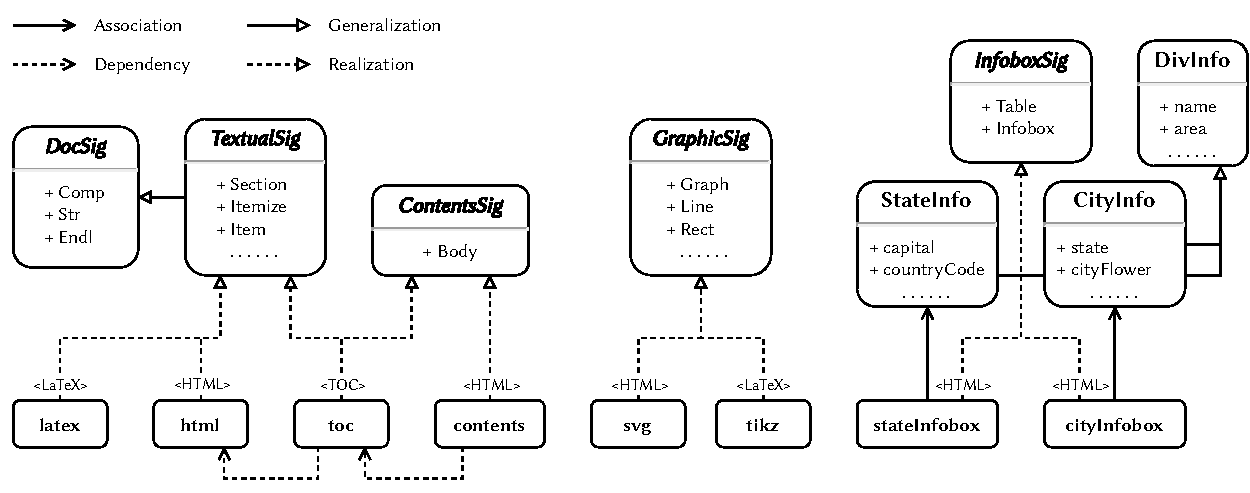
\includegraphics[width=\textwidth]{libraries.pdf}
  \caption{A simplified diagram of \ExT components.} \label{fig:diagram}
\end{figure}

\paragraph{The components of \ExT.}
We have implemented several extensions of \ExT, as shown in
\autoref{fig:diagram}. In the upper part of the diagram, the capitalized names
in a bold italic font (e.g. {\small \sffamily \bfseries \itshape DocSig}) are
compositional interfaces, while those in a bold upright font (e.g. {\small
\sffamily \bfseries DivInfo}) are normal types. The smaller boxes at the bottom
of the diagram are compositional traits. They implement different interfaces
with the sorts specified on the dashed arrows, (e.g. {\small \sffamily <HTML>}).
Specifically, \lstinline{TextualSig} adds a set of common commands for rich
text, such as \lstinline{Section}, \lstinline{Itemize}, \lstinline{Item}, etc.
It extends \lstinline{DocSig} and targets both HTML and \LaTeX.
\lstinline{GraphicSig} is used to draw vector graphics (including lines,
rectangles, circles, etc.), which are supported in HTML and \LaTeX{} via SVG and
Ti\emph{k}Z respectively. \lstinline{InfoboxSig} targets only HTML and adds
Wikipedia-like infoboxes (containing, for instance, information about areas and
populations of states or cities). All these compositional interfaces and traits
can be combined to form a heterogeneous composition. Notably, the implementation
of \lstinline{ContentsSig}, which is used to generate a table of contents,
introduces some non-trivial dependencies (see \autoref{sec:minipedia}).

\subsection{Static Typing} \label{sec:typing}

A major difference of \ExT from other document DSLs is that it is statically
type checked. With static typing, potential type errors can be detected ahead of
time, saving users' time for debugging. For example, when drawing a line using
SVG, we need to use the \lstinline{<line>} element with four numeric coordinates
(\lstinline{x1}, \lstinline{y1}, \lstinline{x2}, and \lstinline{y2}). However,
since additional information of an SVG element is represented as XML attributes,
all of the coordinates have to be quoted as strings instead of numbers. Only
after rendering it with a web browser and opening developer tools can one check
if attributes are valid. In \ExT, we model the line construct like this:

\begin{lstlisting}
type GraphicSig<Graphic> = {
  Line: { x1: Int; y1: Int; x2: Int; y2: Int } -> Graphic;
  -- and more constructors
};
\end{lstlisting}

\noindent
Before rendering lines via SVG, the types of arguments are checked against the
language interface, and invalid values are rejected in advance. Note that the
error messages are reported in terms of the \ExT surface syntax, which is more
friendly to users than some meta-programming techniques, where errors are
reported in terms of the generated code.

When modeling infoboxes and bibliography in \autoref{sec:minipedia}, we also
make use of data types to represent structured information. For example, we use
\lstinline{DivInfo} to model common information required by all political
divisions, as well as two specific types for states and cities respectively,
which extend \lstinline{DivInfo} using intersection types:

\noindent
\begin{minipage}{0.28\textwidth}
\begin{lstlisting}
type DivInfo = {
  name:       String;
  area:       Int;
  population: Int;
  languages: [String];
};
\end{lstlisting}
\end{minipage}
\hfill
\begin{minipage}{0.29\textwidth}
\begin{lstlisting}
type StateInfo =
       DivInfo & {
  countryCode: String;
  religions:  [String];
  -- and more fields
};
\end{lstlisting}
\end{minipage}
\hfill
\begin{minipage}{0.27\textwidth}
\begin{lstlisting}
type CityInfo =
      DivInfo & {
  cityFlower: String;
  timeZone:   String;
  -- and more fields
};
\end{lstlisting}
\end{minipage}

\noindent In this case, there is quite a bit of structure in the data. It
statically describes what fields are allowed and what types these fields have. 
